% fig5_robustez_forest.tex — Forest Plot de Robustez do Gradiente Educacional
% Compilar standalone via: pdflatex fig5_robustez_forest.tex
\documentclass[border=6pt]{standalone}
\usepackage[T1]{fontenc}
\usepackage[utf8]{inputenc}
\usepackage{amsmath,amssymb}
\usepackage{tikz}
\usetikzlibrary{arrows.meta,calc}

% Paleta Institucional
\definecolor{instblue}{HTML}{012169}
\definecolor{instgold}{HTML}{B9975B}
\definecolor{vermillion}{HTML}{D55E00}
\definecolor{gridgray}{HTML}{E5E5E5}
\definecolor{axisgray}{HTML}{4A4A4A}

\begin{document}
% Coordinate map:
% x represents beta_1 in [0.12, 0.34], scaled: X(beta) = (beta - 0.12) * 45
% y represents specifications 1..13 (from bottom to top)
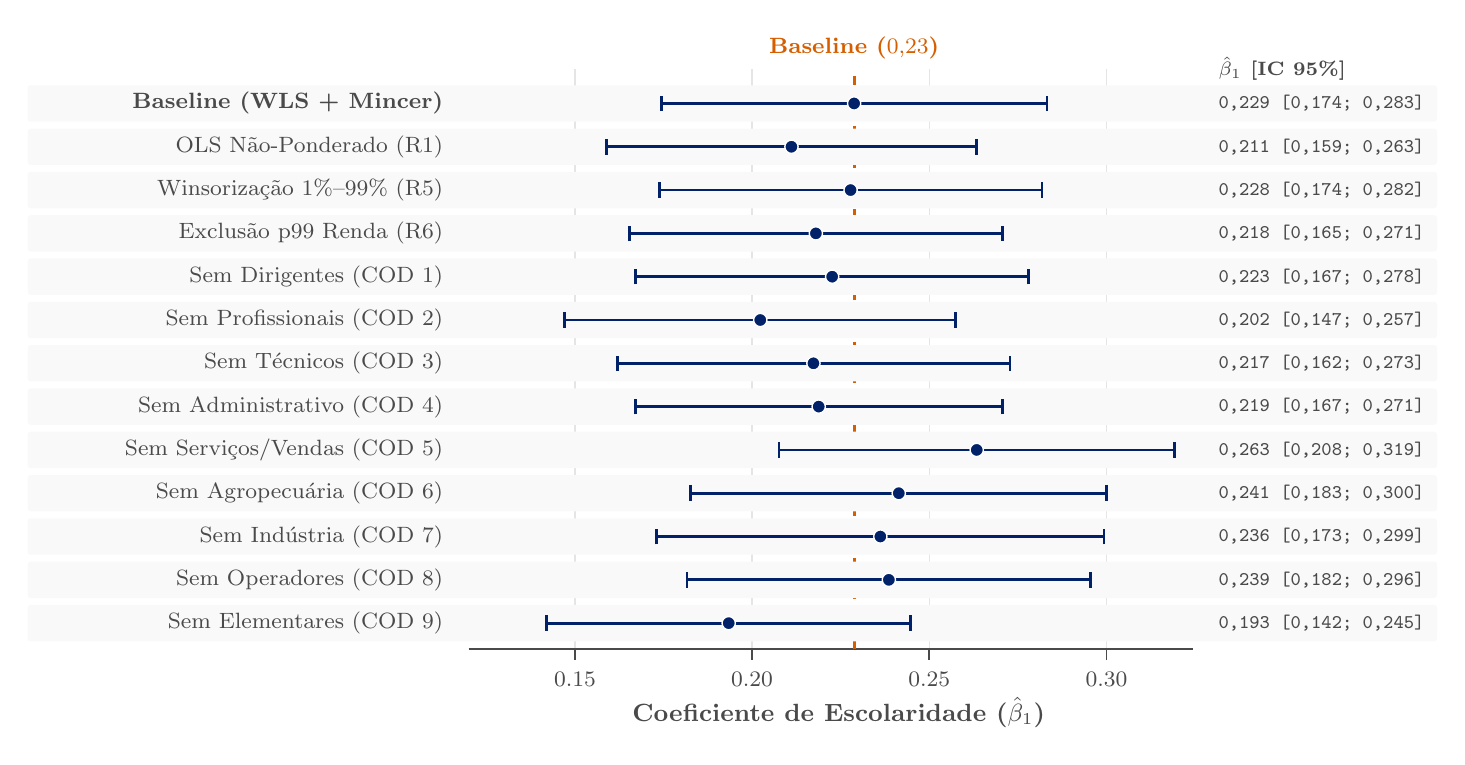
\begin{tikzpicture}[x=1cm, y=0.55cm]

  % Grid lines (vertical)
  \foreach \b/\bx in {0.15/1.35, 0.20/3.6, 0.25/5.85, 0.30/8.1} {
    \draw[gridgray, line width=0.5pt] (\bx, 0.4) -- (\bx, 13.8);
    \draw[axisgray, line width=0.6pt] (\bx, 0.4) -- (\bx, 0.15);
    \node[below, font=\footnotesize, text=axisgray] at (\bx, 0.1) {\b};
  }

  % Axis line and label
  \draw[axisgray, line width=0.8pt] (0, 0.4) -- (9.2, 0.4);
  \node[below=14pt, font=\small\bfseries, text=axisgray] at (4.7, 0.4) {Coeficiente de Escolaridade ($\hat{\beta}_1$)};

  % Baseline reference dashed line (beta = 0.2288 -> X = 4.896)
  \draw[vermillion, dashed, line width=1.0pt] (4.896, 0.4) -- (4.896, 13.8);
  \node[above, font=\footnotesize\bfseries, text=vermillion] at (4.896, 13.8) {Baseline ($0{,}23$)};

  % Data: y / label / beta / ci_lower / ci_upper
  % Scale formula: (val - 0.12) * 45
  \foreach \y/\spec/\bx/\cil/\ciu/\bval/\cival in {
    1/{Sem Elementares (COD 9)}/3.303/0.990/5.616/{0{,}193}/{[0{,}142; 0{,}245]},
    2/{Sem Operadores (COD 8)}/5.337/2.772/7.902/{0{,}239}/{[0{,}182; 0{,}296]},
    3/{Sem Indústria (COD 7)}/5.229/2.385/8.069/{0{,}236}/{[0{,}173; 0{,}299]},
    4/{Sem Agropecuária (COD 6)}/5.463/2.822/8.105/{0{,}241}/{[0{,}183; 0{,}300]},
    5/{Sem Serviços/Vendas (COD 5)}/6.453/3.942/8.964/{0{,}263}/{[0{,}208; 0{,}319]},
    6/{Sem Administrativo (COD 4)}/4.446/2.115/6.777/{0{,}219}/{[0{,}167; 0{,}271]},
    7/{Sem Técnicos (COD 3)}/4.379/1.886/6.876/{0{,}217}/{[0{,}162; 0{,}273]},
    8/{Sem Profissionais (COD 2)}/3.704/1.220/6.183/{0{,}202}/{[0{,}147; 0{,}257]},
    9/{Sem Dirigentes (COD 1)}/4.617/2.120/7.110/{0{,}223}/{[0{,}167; 0{,}278]},
    10/{Exclusão p99 Renda (R6)}/4.410/2.043/6.777/{0{,}218}/{[0{,}165; 0{,}271]},
    11/{Winsorização 1\%--99\% (R5)}/4.851/2.421/7.281/{0{,}228}/{[0{,}174; 0{,}282]},
    12/{OLS Não-Ponderado (R1)}/4.100/1.751/6.449/{0{,}211}/{[0{,}159; 0{,}263]},
    13/{\textbf{Baseline (WLS + Mincer)}}/4.896/2.448/7.344/{\textbf{0{,}229}}/{[\textbf{0{,}174; 0{,}283}]}
  } {
    % Alternating row background for readability
    \fill[gray!5, rounded corners=1pt] (-5.6, \y-0.42) rectangle (12.3, \y+0.42);

    % Spec label on left
    \node[left, font=\footnotesize, text=axisgray] at (-0.2, \y) {\spec};

    % Error bar (CI 95%)
    \draw[instblue, line width=1.0pt] (\cil, \y) -- (\ciu, \y);
    \draw[instblue, line width=1.0pt] (\cil, \y-0.18) -- (\cil, \y+0.18);
    \draw[instblue, line width=1.0pt] (\ciu, \y-0.18) -- (\ciu, \y+0.18);

    % Point estimate
    \filldraw[fill=instblue, draw=white, line width=0.5pt] (\bx, \y) circle (2.4pt);

    % Value annotation on right
    \node[right, font=\scriptsize\ttfamily, text=axisgray] at (9.4, \y) {\bval\ \cival};
  }

  % Header for numbers column
  \node[right, font=\scriptsize\bfseries, text=axisgray] at (9.4, 13.8) {$\hat{\beta}_1$ [IC 95\%]};

\end{tikzpicture}
\end{document}
